\documentclass[a4paper,10pt]{article}%


\usepackage[hidelinks]{hyperref}
\hypersetup{
%  colorlinks,
  linktoc=page
}

\input{commands.tex}%

\author{Peter Bonventre, Lu\'is A. Pereira}%
\title{Genuine equivariant operads}%

\usepackage{showkeys}

\usepackage{stmaryrd}

\usepackage{geometry}

\usepackage{tikz}%
\tikzset{%
  treenode/.style = {shape=rectangle, rounded corners,%
                     draw, align=center,%
                     top color=white, bottom color=blue!20},%
  root/.style     = {treenode, font=\Large, bottom color=red!30},%
  env/.style      = {treenode, font=\ttfamily\normalsize},%
  dummy/.style    = {circle,draw,inner sep=0pt,minimum size=2mm}%
}%

\usetikzlibrary[decorations.pathreplacing]

\begin{document}	\maketitle%





\begin{example}
Let $G=\mathbb{Z}_{/8}$. The following exemplifies a pull back along the twist map $\varphi\colon G/2G \to G/2G$ (i.e., accounting for order, $\varphi$ is the permutation $(12)$), 
with the topmost representation of $\varphi^{\**} T$ maintaining 
the chosen generators for each edge orbit from $T$ and the bottom representation choosing instead the generators to be minimal with regard to the planar structure.
\begin{equation}
	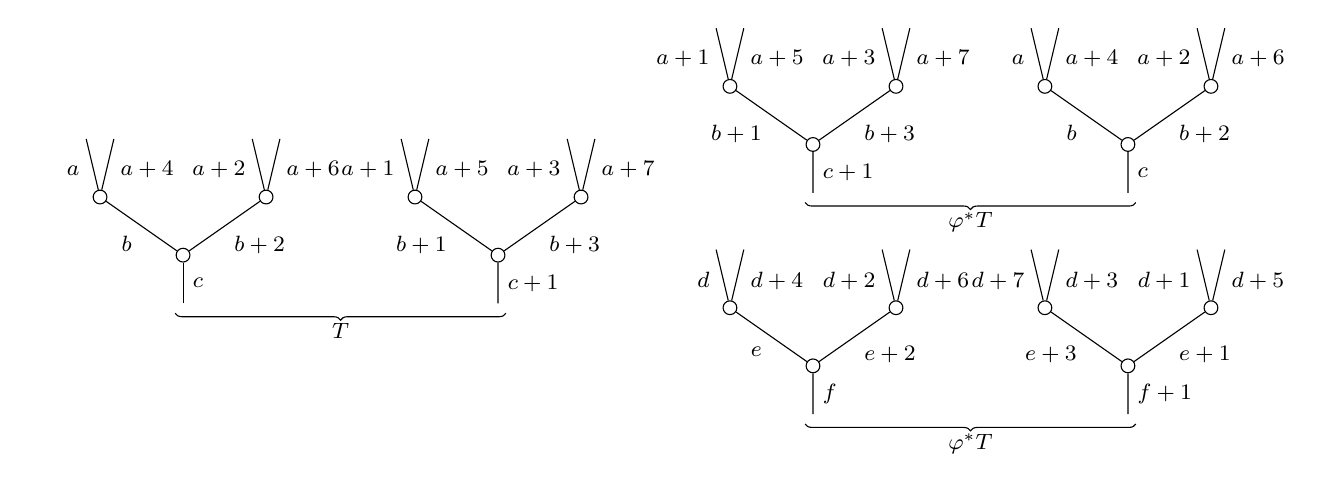
\begin{tikzpicture}[grow=up,auto,level distance=2.1em,every node/.style = {font=\footnotesize},dummy/.style={circle,draw,inner sep=0pt,minimum size=1.75mm}]
		\node at  (0,0) {}
			child{node [dummy] {}
				child[sibling distance = 6em]{node [dummy] {}
					child[sibling distance = 1em]{
					edge from parent node [swap,near end] {$a+6$}}
					child[sibling distance = 1em]{
					edge from parent node [near end] {$a+2$}}
				edge from parent node [swap] {$b+2$}}
				child[sibling distance = 6em]{node [dummy] {}
					child[sibling distance = 1em]{
					edge from parent node [swap,near end] {$a+4$}}
					child[sibling distance = 1em]{
					edge from parent node [near end] {$\phantom{+1}a$}}
				edge from parent node {$b$}}
			edge from parent node [swap] {$c$}};
		\node at  (4,0) {}
			child{node [dummy] {}
				child[sibling distance = 6em]{node [dummy] {}
					child[sibling distance = 1em]{
					edge from parent node [swap,near end] {$a+7$}}
					child[sibling distance = 1em]{
					edge from parent node [near end] {$a+3$}}
				edge from parent node [swap] {$b+3$}}
				child[sibling distance = 6em]{node [dummy] {}
					child[sibling distance = 1em]{
					edge from parent node [swap,near end] {$a+5$}}
					child[sibling distance = 1em]{
					edge from parent node [near end] {$a+1$}}
				edge from parent node {$b+1$}}
			edge from parent node [swap] {$c+1$}};
		\draw[decorate,decoration={brace,amplitude=2.5pt}] (4.1,0) -- (-0.1,0) node[midway]{$T$};
	\begin{scope}[yshift=4em]
		\node at  (12,0) {}
			child{node [dummy] {}
				child[sibling distance = 6em]{node [dummy] {}
					child[sibling distance = 1em]{
					edge from parent node [swap,near end] {$a+6$}}
					child[sibling distance = 1em]{
					edge from parent node [near end] {$a+2$}}
				edge from parent node [swap] {$b+2$}}
				child[sibling distance = 6em]{node [dummy] {}
					child[sibling distance = 1em]{
					edge from parent node [swap,near end] {$a+4$}}
					child[sibling distance = 1em]{
					edge from parent node [near end] {$\phantom{+1}a$}}
				edge from parent node {$b$}}
			edge from parent node [swap] {$c$}};
		\node at  (8,0) {}
			child{node [dummy] {}
				child[sibling distance = 6em]{node [dummy] {}
					child[sibling distance = 1em]{
					edge from parent node [swap,near end] {$a+7$}}
					child[sibling distance = 1em]{
					edge from parent node [near end] {$a+3$}}
				edge from parent node [swap] {$b+3$}}
				child[sibling distance = 6em]{node [dummy] {}
					child[sibling distance = 1em]{
					edge from parent node [swap,near end] {$a+5$}}
					child[sibling distance = 1em]{
					edge from parent node [near end] {$a+1$}}
				edge from parent node {$b+1$}}
			edge from parent node [swap] {$c+1$}};
		\draw[decorate,decoration={brace,amplitude=2.5pt}] (12.1,0) -- (7.9,0) node[midway]{$\varphi^{\**}T$};
	\end{scope}
	\begin{scope}[yshift=-4em]
		\node at  (8,0) {}
			child{node [dummy] {}
				child[sibling distance = 6em]{node [dummy] {}
					child[sibling distance = 1em]{
					edge from parent node [swap,near end] {$d+6$}}
					child[sibling distance = 1em]{
					edge from parent node [near end] {$d+2$}}
				edge from parent node [swap] {$e+2$}}
				child[sibling distance = 6em]{node [dummy] {}
					child[sibling distance = 1em]{
					edge from parent node [swap,near end] {$d+4$}}
					child[sibling distance = 1em]{
					edge from parent node [near end] {$\phantom{+1}d$}}
				edge from parent node {$e$}}
			edge from parent node [swap] {$f$}};
		\node at  (12,0) {}
			child{node [dummy] {}
				child[sibling distance = 6em]{node [dummy] {}
					child[sibling distance = 1em]{
					edge from parent node [swap,near end] {$d+5$}}
					child[sibling distance = 1em]{
					edge from parent node [near end] {$d+1$}}
				edge from parent node [swap] {$e+1$}}
				child[sibling distance = 6em]{node [dummy] {}
					child[sibling distance = 1em]{
					edge from parent node [swap,near end] {$d+3$}}
					child[sibling distance = 1em]{
					edge from parent node [near end] {$d+7$}}
				edge from parent node {$e+3$}}
			edge from parent node [swap] {$f+1$}};
		\draw[decorate,decoration={brace,amplitude=2.5pt}] (12.1,0) -- (7.9,0) node[midway]{$\varphi^{\**}T$};
	\end{scope}
	\end{tikzpicture}
\end{equation}
We note that $(\varphi^{\**}(T))_{v_{G e}} = \psi^{\**}(T_{v_{G b}})$
for $\psi$ the permutation $(13)(24)$ encoded by the composite identifications
$\{1,2,3,4\} \simeq \{e,e+2,e+3,e+1\} \simeq 
\{b+1,b+3,b,b+2\}\simeq \{3,4,1,2\}$.
\end{example}




\begin{example}
\begin{equation}
	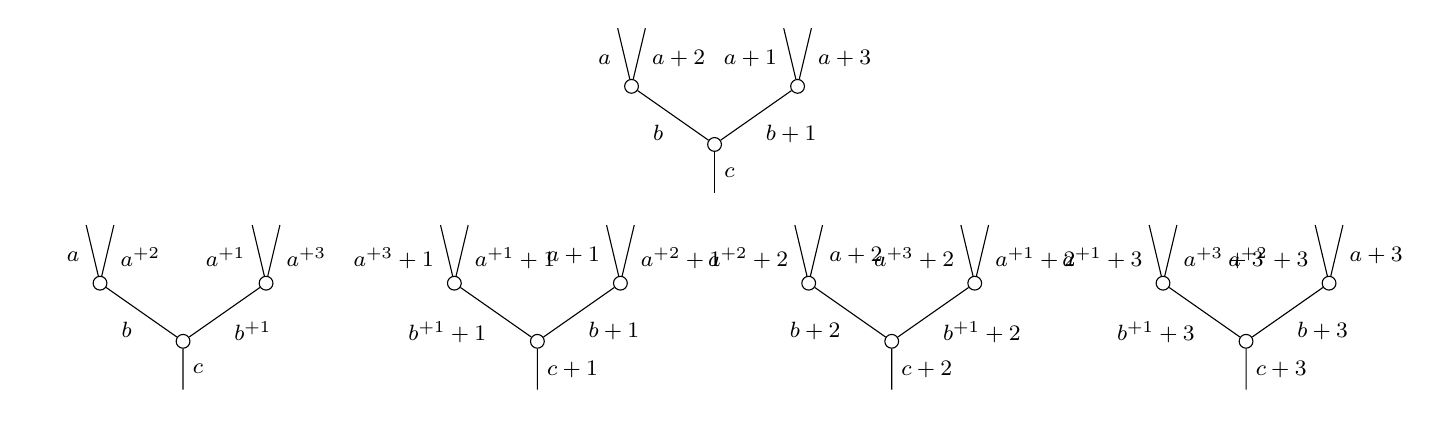
\begin{tikzpicture}[grow=up,auto,level distance=2.1em,every node/.style = {font=\footnotesize},dummy/.style={circle,draw,inner sep=0pt,minimum size=1.75mm}]
		\node at  (0,0) {}
			child{node [dummy] {}
				child[sibling distance = 6em]{node [dummy] {}
					child[sibling distance = 1em]{
					edge from parent node [swap,near end] {$a+3$}}
					child[sibling distance = 1em]{
					edge from parent node [near end] {$a+1$}}
				edge from parent node [swap] {$b+1$}}
				child[sibling distance = 6em]{node [dummy] {}
					child[sibling distance = 1em]{
					edge from parent node [swap,near end] {$a+2$}}
					child[sibling distance = 1em]{
					edge from parent node [near end] {$\phantom{+1}a$}}
				edge from parent node {$b$}}
			edge from parent node [swap] {$c$}};
		\node at  (-6.75,-2.5) {}
			child{node [dummy] {}
				child[sibling distance = 6em]{node [dummy] {}
					child[sibling distance = 1em]{
					edge from parent node [swap,near end] {$a^{+3}$}}
					child[sibling distance = 1em]{
					edge from parent node [near end] {$a^{+1}$}}
				edge from parent node [swap] {$b^{+1}$}}
				child[sibling distance = 6em]{node [dummy] {}
					child[sibling distance = 1em]{
					edge from parent node [swap,near end] {$a^{+2}$}}
					child[sibling distance = 1em]{
					edge from parent node [near end] {$\phantom{+1}a$}}
				edge from parent node {$b$}}
			edge from parent node [swap] {$c$}};
		\node at  (-2.25,-2.5) {}
			child{node [dummy] {}
				child[sibling distance = 6em]{node [dummy] {}
					child[sibling distance = 1em]{
					edge from parent node [swap,near end] {$a^{+2}+1$}}
					child[sibling distance = 1em]{
					edge from parent node [near end] {$a+1$}}
				edge from parent node [swap] {$b+1$}}
				child[sibling distance = 6em]{node [dummy] {}
					child[sibling distance = 1em]{
					edge from parent node [swap,near end] {$a^{+1}+1$}}
					child[sibling distance = 1em]{
					edge from parent node [near end] {$\phantom{+1}a^{+3}+1$}}
				edge from parent node {$b^{+1}+1$}}
			edge from parent node [swap] {$c+1$}};
		\node at  (2.25,-2.5) {}
			child{node [dummy] {}
				child[sibling distance = 6em]{node [dummy] {}
					child[sibling distance = 1em]{
					edge from parent node [swap,near end] {$a^{+1}+2$}}
					child[sibling distance = 1em]{
					edge from parent node [near end] {$a^{+3}+2$}}
				edge from parent node [swap] {$b^{+1}+2$}}
				child[sibling distance = 6em]{node [dummy] {}
					child[sibling distance = 1em]{
					edge from parent node [swap,near end] {$a+2$}}
					child[sibling distance = 1em]{
					edge from parent node [near end] {$\phantom{+1}a^{+2}+2$}}
				edge from parent node {$b+2$}}
			edge from parent node [swap] {$c+2$}};
		\node at  (6.75,-2.5) {}
			child{node [dummy] {}
				child[sibling distance = 6em]{node [dummy] {}
					child[sibling distance = 1em]{
					edge from parent node [swap,near end] {$a+3$}}
					child[sibling distance = 1em]{
					edge from parent node [near end] {$a^{+2}+3$}}
				edge from parent node [swap] {$b+3$}}
				child[sibling distance = 6em]{node [dummy] {}
					child[sibling distance = 1em]{
					edge from parent node [swap,near end] {$a^{+3}+3$}}
					child[sibling distance = 1em]{
					edge from parent node [near end] {$\phantom{+1}a^{+1}+3$}}
				edge from parent node {$b^{+1}+3$}}
			edge from parent node [swap] {$c+3$}};
	\end{tikzpicture}
\end{equation}
\end{example}












\bibliography{biblio}{}



\bibliographystyle{abbrv}



\end{document}